\chapter{Background}\label{chap:background}
This section gives an overview of the SGM and related work on its optimization. Furthermore, the used optimizers in our experiments are explained.
\section{The Skip-Gram Model}
The SGM is a very simple model used to learn WE. The idea is to train the model, a neural network, on a fake task and then use some of the weights of the neural network as embeddings. To understand this fake task center and context words must be defined. The center word is any given word in a sentence, from which we want to learn the WE. The context words of this specific center word are the words left and right in a given window $m$ in the sentence. See Figure \ref{fig:window_ex} as an example, where the context words are highlighted. An important thing to notice, is that instead of having a fixed window size $m$, each word will randomly have a window size between $1$ and $m$. The idea behind having different window sizes is that words that are further away in the sentence, have less semantic correlation to the center word.

\begin{figure}[h]
\centering
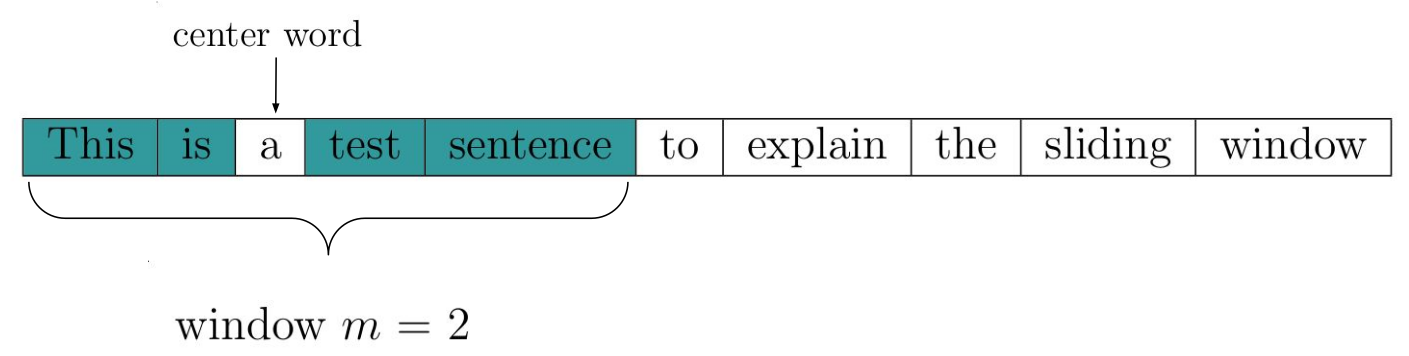
\includegraphics[scale=0.3]{images/window_ex}
\caption{Example of a center word and it's context words}
\label{fig:window_ex}
\end{figure}
%TODO think about example matrix
With these definitions the fake task can be defined: given a pair of center and context words, which will be our training samples, the goal of the network is to predict the probability of each word to appear in the context of the center word. One may ask how such a network is built. The network consists of two matrices, a projection and an output layer. Both of these matrices store word embeddings. The first one, the projection layer, will store the WE for one specific word in one specific row. It will have dimension $T\times d$, with $T$ being the size of our vocabulary and $d$ the dimension of our WE. The second layer, the output layer, will store one WE in each column. The idea behind these 2 layers is that the input layer will represent our words as center word and the output layer as context words. Since the task of the network being to predict the probability of each word appearing in the context of a given center word, the following probability should be maximized:\\
\begin{equation} \label{eq:basicSkip}
\prod_{t=1}^T \prod_{-m<j<m} p(w_{t+j}|w_t)
\end{equation}
Where T is the number of words in the corpus data, $w_t$ the $t^{th}$ word in the corpus data and $m$ is the context window. This means that the $m$ nearest words to $w$ are considered as context words.
Equation \ref{eq:basicSkip} can be transformed into sums by using log probabilities:
\begin{equation}
\sum _{t=1}^T \sum_{-m<j<m} log( p(w_{t+j}|w_t) )
\end{equation}
where the parameters are the same as in Equation \ref{eq:basicSkip}.

The basic Skip-Gram Model uses a classical Softmax to calculate the conditional probability $p(w_{t+j}|w_t)$:
\begin{equation} \label{eq:softmax}
p(w_{t+j}|w_t)= \frac{exp( \tilde{v}_{w_{t+j}}^Tv_{w_t})}{\sum_{w=1}^v exp(\tilde{v}_w^Tv_{ w_t})}
\end{equation}

Here $\tilde{v}_{w_t}$ and $ v_{w_t}$ are the vector representations, stored respectively in the projection Layer (first Matrix) and in the output layer (second Matrix). There is a problem with the classical softmax. As a matter of fact, it is unsuitable to compute the softmax. For the computation of $\sum_{w=1}^v exp(\tilde{v_w}^T w_t)$, the denominator in Equation \ref{eq:softmax}, one has to go over the whole corpus data. As very big data sets are needed to train the model, this is not a solution. Mikolov et al. \cite{mikolov2} proposed different solutions. The first solution is to use a Hierarchical softmax introduced by Morin and Bengio \cite{hsoftmax}. In this model, the probability distribution of the output nodes is saved in a binary tree which gives one a logarithmic computation time for each of these probabilities and makes it suitable to compute the softmax. Another possibility is the use of negative sampling which is discussed in the next section.

\section{Negative Sampling}
A second alternative solution to the use of a classical softmax is negative sampling. Negative Sampling is a simplification of Noise Contrastive Estimation (NCE) which was introduced by Gutmann and Hyv{\"a}rinen \cite{nce-original}, and first applied to NLP by Mnih and Teh \cite{mnih}. This section will shortly describe NCE and then how Mikolov et al. \cite{mikolov2} simplified it to create the technique called negative sampling. \\ The idea behind NCE is to distinguish data from noise. It does so by reducing the problem to a logistic regression task and does it by maximizing the log probability. The SGM is only interested in good word representation, hence the probability of the word is not meaningful as long as the quality of the word representations remains high. Mikolov et al. \cite{mikolov2} simplified NCE and called it Negative Sampling, which will be explained next.\\
The main goal of negative sampling is to only update the output nodes of certain words. This will obviously save an enormous amount of computation time. The idea is that given a pair $(c,w) \in D$, where $c$ is a word in the context window of $w$ we select $K$ random words $k_i$ from the corpus data $D$. We assume those words do not appear in the context of $w$. We denote the score that the $(c,w)$ wasn't drawn at random the following way: $p(y=1|c,w)$, and if $(k,w) $ is chosen at random this way: $p(y=0|k,w)$. Now we use logistic regression to update the weights of the $k$ selected context words and $c$. By doing so we will only have to update $k+1$ nodes.

Let's look at how we construct our objective function for a given word $w$ and one of its context words $c$:

\begin{align*}
p(c|w) &= p(y=1|c,w) + \prod_{k\in K} p(y=0|k,c)
\\&= p(y=1|c,w) + \prod_{k\in K} 1- p(y=1|k,c)
\\&= log((p(y=1|c,w)) + \sum_{k\in K} log(1- p(y=1|k,c))
\\&= log(\frac{1}{1+e^{-v_c \tilde{v_w }}}) + \sum_{k\in K} log(1-\frac{1}{1+e^{-v_c \tilde{v_k}}})
\\&= log(\frac{1}{1+e^{-v_c \tilde{v_w } }}) + \sum_{k\in K} log(\frac{1}{1+e^{v_c \tilde{v_k} }})
\\&= log(\sigma(v_c \tilde{v_w } ) + \sum_{k\in K} \sigma(log(-v_c \tilde{v_k} )) &&\text{where, $\sigma(x) = \frac{1}{1+e^{-x}}$}
\end{align*}\label{eq:obj_neg_samples}

Where $v_c$ and $\tilde{v_w }$, can be interpreted as before in Equation \ref{eq:softmax}. The goal is to maximize this objective function. Another way to look at this function, apart from logistic regression, and understand why it's working so well, is to assume that two vectors are similar if their dot product is high. Therefore, we maximize the dot product of similar words $(w,c)$ ($c$ appears in the context of $w$) and minimize it for dissimilar words $(w,k_i)$ (those were selected randomly).
We see that to compute our objective function we will only have to compute the sum over the number of negative samples $K$, which is very small in practice (2-20). To put things in perspective lets imagine our data set consists of 100000 words, we set $K=2$. Assume each output neuron has a weight vector $v$ with $|v| = 300$. In consequence, when updating our weights we would only update $0.2*10^{-2}$ of the 300 million weights in the output layer.

One question remains: how do we choose our random words? Mikolov et al. \cite{mikolov2} used the following unigram distribution:

\begin{equation} \label{eq:unigram}
P(w)=\frac{f(w)^{\frac{3}{4}}}{\sum_{t=0}^{T} f(w_t)^{\frac{3}{4}}}
\end{equation}
where $f(w)$ is the frequency of $w_t$. The value of $\frac{3}{4}$ is set empirically. Raising the unigram distribution to power of $\frac{3}{4}$ makes it less likely for a word to be drawn if it often appears in the dataset in comparison to the basic unigram distribution. See figure \ref{fig:frequency_ex} for an example.
\begin{figure}[ht]
\centering
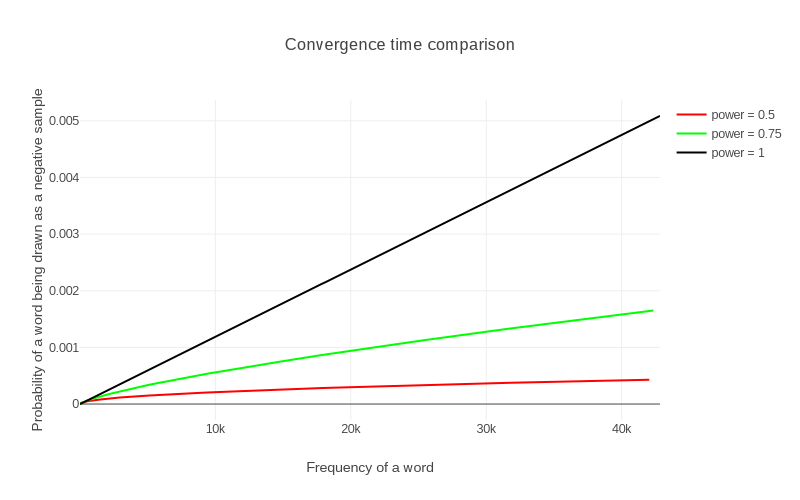
\includegraphics[scale=0.45]{images/frequency_ex}
\caption{Probabililty of a word, of the text8 dataset (sampled), to be chosen at random according to its frequency and the power to which the unigram distribution is raised}
\label{fig:frequency_ex}
\end{figure}
It's quite easily observable that this approach will outperform the classical softmax in computation time, as it only compute the sum over $K$ output nodes. Now the question arises if the accuracy is good enough but according to Mikolov et al. \cite{mikolov2} the negative sampling method "is an extremely simple training method that learns accurate representations". As a matter of fact, Mikolov et al. \cite{mikolov2} reported a 6\% accuracy improvement in comparison to a Hierarchical Softmax model. Therefore, it is a good solution to the problem raised by the classical softmax.
We now have enough background knowledge about the SGM to look at how it can be optimized. The next section introduces earlier approaches to optimize the SGM.

\section{Optimization of the Skip Gram Model}
Due to the popularity of the SGM, a lot of research went into optimizing it. This research can be divided into two categories, optimization of the throughput and the optimization of the algorithm's accuracy. The latter was achieved by allowing words to have multiple meanings, also called context-sensitive word embedings. For our work, the optimization of the throughput is of big interest while the semantic optimization is aimed at giving the reader a more holistic comprehension of the possible research directions.
This section will first give an overview of the optimization of the throughput and then present one paper that focused on context-sensitive word embeddings.

\subsection{Optimization of the throughput}

In the original model, the optimization is done with Stochastic Gradient Descent (SGD), which is a sequential algorithm. This process does not favor parallelization. To deal with this specific problem Mikolov et al.\cite{mikolov2} used a Hogwild tree proposed by Recht et al.\cite{hogwild}. The approach is to allow multiple threads to access a shared memory, in this case, the single model. In the original SGM, the threads are constructed as follows: at the beginning of training, the dataset is split into $N$ evenly sized chunks and each of these chunks will be processed by a one thread. The threads run parallel and have access to the shared memory. Therefore, overwriting errors are bound to happen. According to Recht et al.\cite{hogwild} the overwriting errors won't lead to a significant accuracy loss if the data is sparse enough. But in the case of NLP, the problem seems to be a bit more significant, and especially for word embedding, as many words share the same context words. There were several attempts at solving this issue, and we are going to cover a few of them in the following subsections.

\subsubsection{Parallelization by the use of caching}
This idea was proposed by Vuurens et al. \cite{efficient}. The architecture used here is the basic skip gram model with a hierarchical softmax. The general idea is to cache the most frequently used nodes of the binary tree used to memorize the probability distribution and update them on the shared single model after a certain number of seen words (the paper used the number 10). The paper produced interesting results as they managed to decrease execution time by increasing the number of cores used for the calculation. This is very powerful because in the original implementation the execution time regressed after using more than 8 cores. It seems to indicate that too much overwriting was happening, as the number of concurrent threads surpasses a certain threshold. This can be seen in Figure \ref{fig:efficient}, where c31 is the model proposed by Vuurens et al.\cite{efficient}. The model did not suffer any accuracy loss in comparison to the original SGM model.
\begin{figure}[ht]
\centering
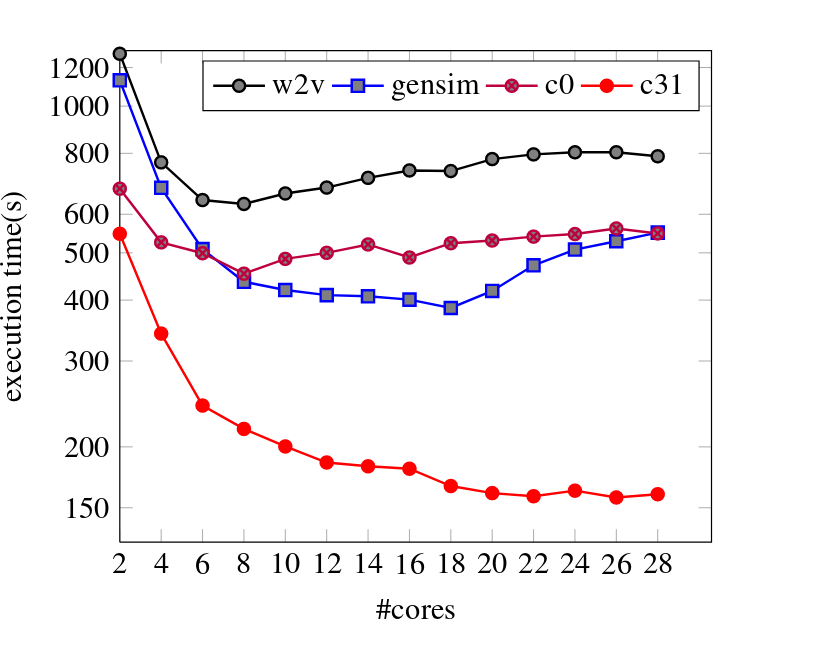
\includegraphics[scale=0.3]{images/cachingEfficiency.png}
\caption{Comparasion of the execution time in relation to the number of used cores \cite{efficient}}
\label{fig:efficient}
\end{figure}
This work proposes a very good way to parallelize the SGM, as in particular, it allows using more cores during the computation. As this approached focused on the Hierarchical softmax, in contrast to our work which used negative sampling, the next section covers optimizations of the Skip-Gram Model with negative sampling(SGNS).

\subsubsection{Parallization in shared and Distributed Memory}
The first parallelized solution which was proposed by Ji et al. \cite{intel}, is to try to reduce the cost of our vector multiplication. The main idea in this paper is to convert the level 1-BLAS (Basic linear subprogram) vector to vector operations to a level 3-BLAS matrix multiplication operation, which are efficiently implemented into hardware and consequently faster. This is achieved, by using the same negative samples for each context word of a given word $w$. Instead of using for each context word a vector to vector multiplication we can transform this into a matrix multiplication, under the assumption that we will not lose accuracy by sharing the same negative samples. The matrix multiplication can be represented in the following way.
\[
\begin{bmatrix}
w \\
w_{n_1} \\
\vdots \\
w_{n_k}\\
\end{bmatrix}
*
\begin{bmatrix}
w_{c_1}\\
\vdots\\
w_{c_{2m}}\\
\end{bmatrix}
\]

where $w$ is our given word, $w_{n_1}...w_{n_k}$ are the shared negative samples, with $k \in [5,20]$, and $w_{c_1}...w_{c_2m}$ are the words inside of the context window $m$ of $w$, with $m \in [10,20]$, also called a batch of input context words. After each batch the model updates the weights of the used vectors.
This model achieves a 3.6 fold increase in throughput, by only losing 1\% of accuracy. An aspect that is not as useful to us is that the experiments were done on CPU, as modern GPU's are often used in many machine learning libraries, as with CUDA for example, there still need work to be done to optimize it with GPU's. This was done by Seulki and Youngmin \cite{gpu}, which is described in the next section.

\subsubsection{Accelleration of word2vec by Using GPU's}
Seulki and Youngmin \cite{gpu} focused on getting a better throughput on the SGM when using GPU's. As the SGM is a sequential algorithm, is is not easy to parallelize it, especially if one wants to parallelize the training of individual training samples. As the algorithm goes sequentially over a sentence, the samples next to each other, in order of execution, will almost every time have the same input word. Consequently, it's very hard to parallelize at this level. To solve this problem, Seulki and Youngmin \cite{gpu} proposed the idea to parallelize the update of each dimension of the word embedding, since those are completely independent of each other. They achieved this by mapping each dimension to a CUDA thread while mapping each sentence to a CUDA block. As each CUDA block runs independently, the training of the sentences is parallelized, and the fact that sentences have different length is of no problem. If the execution time of the GPU kernel is greater than time used to read the sentences, it could be a smart choice to use multiple GPU's. According to Seulki and Youngmin \cite{gpu}, if multiple GPU's are used, there is a need for synchronizing the model, which will hinder run time performance. They achieved their best results with 2 concurrent GPU'S. The accomplished results were very good as they managed a 20x speedup compared to a single threaded CPU execution, which is a 3x increase in comparison to the original C code from Mikolov et al. \cite{mikolov2}, with no loss in accuracy. The problem with this and all the above optimization is that the code is not easily available. Therefore, we need an optimized implementation of the SGM that is easily available. This is provided by Gensim \cite{gensim}, which will be outlined in the next section.
%%%%%%%%%%%
\subsubsection{Gensim}
Gensim \cite{gensim} is a pure Python library that holds a state of the art implementation of the SGM. Gensim is written in Cython, which first allowed Gensim to have the same runtime as the original C code. Furthermore, it made use of BLAS's and precomputed sigmoid tables, while also trying to parallelize the training of different sentences. This finally yielded in a 4x speedup in run time. Gensim is an important tool as it allows us, as a python library, to compare our data rather easily. It was also used in related work \cite{intel} and is therefore of value, as it allows to us compare our work in a simpler way. This concludes our overview of the optimizations of the throughput of the SGM. In the next section, we give a quick outlook of what has been done in the field of context-sensitive word embeddings.

\subsection{Context sensitive word embedding}
A word has different meanings dependent on its context. This is a problem that is not addressed by the SGM. Some new models, that have taken this issue into consideration, were proposed. A lot of work has been done in this direction, Liu et al.\cite{topicalWE} and Bartunov et al.\cite{breaking} for example, but the one reporting the best results is Liu et al. \cite{contextWithTensor}. The concept of this approach is to change the way we compute the objective function and variables we use in our conditional probability. The idea is to look if a word given a certain context word matches to a topic. \textit{Bank} would match to \textit{finance} given the context word \textit{money}. \textit{Bank} would also match to \textit{nature} if \textit{river} was the given context word. But \textit{Bank} would not match to \textit{nature} with the context word \textit{money}. Now one could ask how to achieve such a context sensitive word embedding? First, we have to introduce new variables, therefore let's look at the objective function used:
\begin{equation}
J(\Omega) = \sum_{(w,t,c)\in D} \sum_{(w,\tilde{t},\tilde{c} \in{\tilde{D}})} max(0,1- g(w,t,c) + g(w,\tilde{t},\tilde{c})) \lambda||\Omega||_{2}^2
\end{equation}

This approach uses the same negative sample technique as described in the previous sections, $D$ is the corpus data and $\tilde{D}$ is the set of negative samples and $\lambda$is the hyper parameter used for the standard $L_2$ standardization. What is interesting here is the function $g(w,c,t)$, where $w$ is a word, $c$ the context word, and $t$ the context in which the word appears. $g$ is defined as follows:
\begin{equation}
g(w,c,t) = u^T \sigma(w^TM^{[1:k]}t+V_c^T(w \oplus t) + b_c)
\end{equation}
where, $u, V_c, b_c$ are standard parameters for a neural network. $\oplus$ is the vector concatenation. The most important parameter is $M^{[1:k]}$, which is a tensor layer, the tensor layer is used because of its ability to model multiple interactions in the data, as this will be useful for multiple contexts. They used SGD for the optimization of this objective function. They achieved interesting results as shown in \ref{fig:multipleContext}.\\
\begin{figure}[ht]
\centering
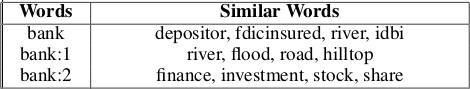
\includegraphics[scale=0.7]{images/multipleContext.png}
\caption{"Nearest neighbor words model and Skip-
Gram. The first line in each block is the results of Skip-Gram;
and the rest lines are the results of our model" \cite{contextWithTensor}}
\label{fig:multipleContext}
\end{figure}

This will conclude our overview of the related work. We will now give the reader an outline of the different Gradient Descent Optimizer used in our experiments.
\section{Gradient Descent Optimizers} \label{optimizers}
The goal of learning in machine learning is to minimize an objective function $J(\theta)$, where $\theta$ is the set of all parameters in our model. This happens by updating the parameters $\theta$ at every training time step $t$. We will denote $\theta_{t}$ as the parameters of our model at the $t^{th}$ time step. In this work, we only examine gradient descent algorithms.
\subsection{Gradient Descent}
The idea in gradient descent optimization is to follow the path of the steepest descent in the shape of the objective function. To get information about the shape of the objective function, one has to compute the gradients of all our parameters $\nabla J(\theta_{t})$, where $J$ is our objective function, and $\theta$ all of our parameters, $t$ denotes the time step at which the parameters are taken. We will define $g_{t}$ as the gradients of our parameters $\theta_t$ according to our objective function $J$. To follow the path of the steepest descent we will have to subtract a portion of this term from our parameter. The magnitude of the portion is often referred to as the learning rate, denoted as $\eta$. For illustration, this means that the gradients will give the direction of the optimization step, whereas the learning rate will give the amplitude of that step. An update at time step $t$ will result in the following equation:
\begin{equation}
\theta_t = \theta_{t-1} - \eta g_{t-1}
\end{equation}
Where all the variables can be interpreted as above. This will also be the case for further Equations.
There are three main variations of Gradient Descent, they differ at the moment they chose to update the parameters.
\subsubsection{Stochastic Gradient Descent (SGD)}
In this variant, the model will update the parameters after each training sample. The problem with this approach is that the variance of the direction of the training step will be very high, as each sample will influence the step individually.

\subsubsection{Batch Gradient Descent}
Here the update of the model happens after having gone through the entire dataset. The problem with this approach is that one updates the model way to infrequently which will lead to a high convergence time.
\subsubsection{Mini-Batch Gradient Descent}
Here on updates the model after having gone through a specific number of training samples. The idea is that the batch will be representative of the entire dataset, which will allow the model to learn quicker, as the updates are more frequent (in comparison to batch gradient descent) and less variant (in comparison to SGD).

\subsubsection{Problems with Gradient Descent Algorithms}
SGD, though it's simplicity, is very limited, therefore some issues appear:

\begin{itemize}
\item The learning parameter is yet another hyper parameter to tune, as the optimum setting will largely vary depending on the training task and architecture of the network
\item Learning rate schedules, that diminish the learning rate as the training progresses, are a commonly accepted technique to improve accuracy. This schedule is most often set at the beginning of the training and will be completely independent of the training set.
\item Every parameter has the same learning rate
\end{itemize}
To tackle those issues numerous advanced optimizers were developed. They will be covered in the next sections.

\subsection{Momentum}
Momentum is a technique used to address one of SGD weak points. As a matter of fact, because SGD can have trouble computing the optimum of objective function that is only steep in one direction. The problem here is that SGD often oscillates in the direction that is not very steep, and only takes small steps in the steep direction. This issue is addressed by SGD with momentum.

It does so by adding a percentage of the last update vector to the current update vector. By doing so the gradient that goes in the same direction will get bigger (building momentum) and gradients that go in different directions will annul themselves.
At the update $t$ we will compute our update vector $v_t$ the following way:
\begin{equation}
v_t = \gamma v_{t-1} + \eta \nabla J (\theta)
\end{equation}\label{eq:momentum}
Where $v_t$ and $v_{t-1}$, respectively are the current and the last update vector, and $\gamma$ a hyper parameter, usually set to $0.9$, that defines the importance of the momentum term. We then update our weights as usual: $\theta_t = \theta_{t-1} - v_t$
\subsection{Nesterov}
Momentum can be a powerful tool, but sometimes be its own enemy. With Momentum, the learning algorithm often overshoots and blows by the Optima. Hence, it will never converge. This problem was addressed by Yurii Nesterov \cite{nesterov}. The idea behind his algorithm is to incorporate the momentum in the computation of our gradients. We will subtract the previous update vector, or just a fraction, from our parameters before computing the gradients. Therefore, we will compute the gradients of the position where we would be with momentum, which will allow us to make a step in a better direction. The computation of the update vector will look the following way:
\begin{equation}
v_t = \gamma v_{t-1} + \eta \nabla J (\theta - \gamma v_{t-1})
\end{equation}

Where the parameters as the same used with momentum in equation \ref{eq:momentum}. SGD with momentum and Nesterov accelerated gradient (NAG) has shown tremendous results in RNN's. But some earlier mentioned problems still remain. NAG, still treats every parameter the same way. Therefore, we need a more complex optimization algorithm, that takes the frequency of a feature into account. Adagrad does just that.

\subsection{Adagrad}\label{ssec:adagrad}
Adagrad \cite{adagrad} is an optimizer that tries to apply different learning rates to different parameters, according to their frequency. The idea is to give very frequent features a small learning rate, and very sparse features a high learning rate. This can be very important for our task of word embeddings, as rare words in the corpus are more important than very frequent ones. As a matter of fact, Pennigton et al. used this algorithm for their training of Glove \cite{glove}, another word embedding system. \\
Each parameter $\theta_i$, at time step $t$ will have it's own learning rate $\eta_{t,i}$
\begin{equation}
\eta_{t,i} = \frac{\eta_0}{\sqrt{\sum^{t}_{i=1} g^{2}_{t,i}} \epsilon}
\end{equation}
where$g_{t,i} = \nabla J(\theta_{t,i})$ is the partial derivative of the loss function with respect to the parameter $\theta_i$ at time step $t$, and $\epsilon$ is a smoothing factor, so that one does not divide by $0$, at the beginning of the computation and $\eta_0$ is the global learning rate.\\ We see that each parameter $\theta_{i}$ has it's one learning rate. For a very frequent feature the sum of the previous square gradients will be very high, hence the learning rate low. This is how Adagrad achieves a different learning rate for each feature.
Consequently, we have $ \theta_{t,i} = \theta_{t-1,i} - \eta_{t-1,i} g_{t-1,i} $, and we can now construct our global parameter update as follows:
\begin{equation}
\theta_{t,i} = \theta_{t-1,i}- \frac{\eta}{\sqrt{G_{{t-1}_{i,i}}} + \epsilon} g_{t-1,i},
\end{equation}

With $G_{t_{i,i}}$ being the diagonal Matrix of the sum of the squares of the gradients ($g_{t,i}^2 $).
There lies one weakness in this approach: the sum of the squares of the previous gradients grows constantly. This means that after a certain number of epochs the learning rate will be insufficient, to update the model. This issue was addressed by the Adadelta algorithm, that will be covered in the next session.

\subsection{Adadelta}\label{ssec:adadelta}
Adadelta \cite{adadelta} not only solves the constantly growing sum problem, but also the fact that one does not have to tune the learning rate by not having one. The gist of Adadelta is that instead of taking all the gradients to compute the sum we will only take a fixed number $w$ of gradients. But instead of inefficiently storing w gradients we will take the exponentially decaying average of the squared gradient, denoted $E[g^{2}]$. The average at time step $t$ will be computed in the following way:
\begin{equation}
E[g^2]_t = \gamma E[g^2]_{t-1} + (1 - \gamma) g^2_t
\end{equation}
where $\gamma$ is a hyper parameter similar to the one used in momentum, that decides how much the past is weighted in contrast to the current gradient. Since Adadelta is an extension of Adagrad the square root of $E[g^{2}]$ is needed which become the Root Mean Squared (RMS) Error:
\begin{equation}
RMS[g]_t = \sqrt{E[g^2]_t + \epsilon}
\end{equation}
Which gives us the following update rule:
\begin{equation}
\theta_t = \theta_{t-1} - \frac{\eta}{RMS[g]_t}g_t
\end{equation}
Here we have two problems, first, the learning rate is still a hyper parameter. And the units do not match. This is a problem Mathew Zeiler wanted to address. That if the parameters would have units the update parameters units would match.
Therefore, they define the exponentially decaying average of squared parameter updates:
\begin{equation}
E[\Delta \theta^2]_t = \gamma E[\Delta \theta^2]_{t-1} + (1 - \gamma) \Delta \theta^2_t \ \ \ \ \ \ \hfill \text{,where } \Delta \theta = - \frac{\eta}{RMS[g]_t}g_t
\end{equation}
As before we can know us the root mean squared error:
\begin{equation}
RMS[\Delta \theta]_{t} = \sqrt{E[\Delta \theta^2]_t + \epsilon}
\end{equation}
As at time step $t$ $RMS[\Delta \theta]_{t} $ is unknown, we approximate it with $ RMS[\Delta \theta]_{t}-1$. Now we replace $\eta$ with $ RMS[\Delta \theta]_{t}-1$ and get the final update rule:
\begin{equation}
\theta_{t+1} = \theta_t - \dfrac{RMS[\Delta \theta]_{t-1}}{RMS[g]_{t}} g_{t}
\end{equation}
\subsection{Adam}
Adaptive Moment Estimation (Adam) \cite{adam}, is a more recent optimization algorithm. It also computes adaptive learning rates. In comparison to Adagrad and Adadelta, it does not only take into consideration the decaying average of the previous squared gradients but also the decaying average of the past gradients.
Let's introduce :
\begin{equation}
m_t = \beta_1 m_{t-1} + (1- \beta_1) g_t
\end{equation}
as the decaying average of the previous gradients, with $\beta_1$ being a hyper parameter similar to $\gamma$ in the previous optimizers, and
\begin{equation}
v_t = \beta_2 v_{t-1} + (1- \beta_2) g^2_t
\end{equation}
as the decaying average of the previous squared gradients, with $\beta_2$ having the same role as $\beta_1$ \\
One problem arises when using this formula, $m_t$ and $tv_t$ are initialized as vectors of zero. Therefore, they are biased towards zero. In consequence, a bias corrected version was introduced:\\
\begin{equation}
\tilde{m_t} = \frac{m_t}{1-\beta^t_1}
\end{equation}
\begin{equation}
\tilde{v_t} = \frac{v_t}{1-\beta^t_2}
\end{equation}
The general update is done exactly in the same way as in Adadelta:
\begin{equation}
\theta_{t} = \theta_{t-1} - \frac{\eta}{\tilde{v_{-1}}+ \epsilon} \tilde{m_{t-1}}
\end{equation}
with $\epsilon$ as a smoothing factor and $\eta$ as the global learning rate. This concludes our overview of gradient descent optimizers, and more generally our background chapter. In the next chapter the reader will be given an outline of our implementation of the Skip-Gram Model.